% Created by tikzDevice version 0.12.3.1 on 2023-03-10 12:26:09
% !TEX encoding = UTF-8 Unicode
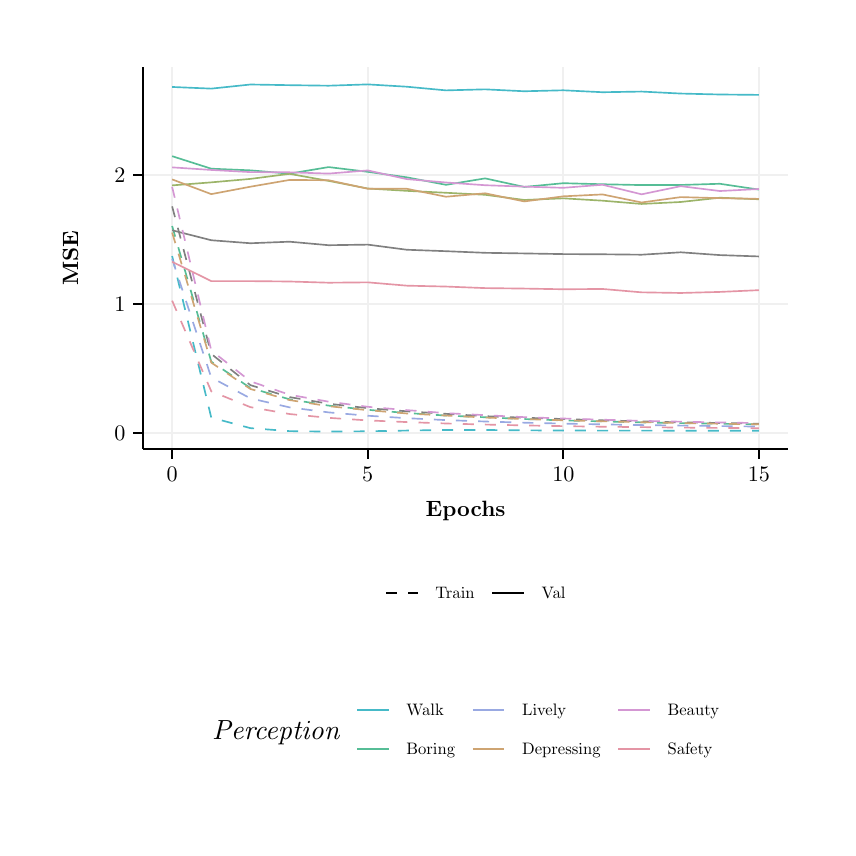
\begin{tikzpicture}[x=1pt,y=1pt]
\definecolor{fillColor}{RGB}{255,255,255}
\path[use as bounding box,fill=fillColor,fill opacity=0.00] (0,0) rectangle (289.08,289.08);
\begin{scope}
\path[clip] (  0.00,  0.00) rectangle (289.08,289.08);
\definecolor{fillColor}{RGB}{255,255,255}

\path[fill=fillColor] (  0.00,  0.00) rectangle (289.08,289.08);
\end{scope}
\begin{scope}
\path[clip] ( 41.60,136.85) rectangle (274.85,274.85);
\definecolor{fillColor}{RGB}{255,255,255}

\path[fill=fillColor] ( 41.60,136.85) rectangle (274.85,274.85);
\definecolor{drawColor}{gray}{0.94}

\path[draw=drawColor,line width= 0.7pt,line join=round] ( 41.60,142.68) --
	(274.85,142.68);

\path[draw=drawColor,line width= 0.7pt,line join=round] ( 41.60,189.32) --
	(274.85,189.32);

\path[draw=drawColor,line width= 0.7pt,line join=round] ( 41.60,235.96) --
	(274.85,235.96);

\path[draw=drawColor,line width= 0.7pt,line join=round] ( 52.20,136.85) --
	( 52.20,274.85);

\path[draw=drawColor,line width= 0.7pt,line join=round] (122.89,136.85) --
	(122.89,274.85);

\path[draw=drawColor,line width= 0.7pt,line join=round] (193.57,136.85) --
	(193.57,274.85);

\path[draw=drawColor,line width= 0.7pt,line join=round] (264.25,136.85) --
	(264.25,274.85);
\definecolor{drawColor}{RGB}{70,186,200}

\path[draw=drawColor,line width= 0.6pt,dash pattern=on 4pt off 4pt ,line join=round] ( 52.20,206.54) --
	( 66.34,148.19) --
	( 80.48,144.37) --
	( 94.61,143.29) --
	(108.75,143.12) --
	(122.89,143.24) --
	(137.02,143.49) --
	(151.16,143.71) --
	(165.30,143.70) --
	(179.43,143.57) --
	(193.57,143.50) --
	(207.71,143.48) --
	(221.84,143.47) --
	(235.98,143.43) --
	(250.11,143.41) --
	(264.25,143.40);

\path[draw=drawColor,line width= 0.6pt,line join=round] ( 52.20,267.65) --
	( 66.34,267.05) --
	( 80.48,268.54) --
	( 94.61,268.30) --
	(108.75,268.11) --
	(122.89,268.58) --
	(137.02,267.74) --
	(151.16,266.42) --
	(165.30,266.79) --
	(179.43,266.10) --
	(193.57,266.45) --
	(207.71,265.75) --
	(221.84,265.99) --
	(235.98,265.27) --
	(250.11,264.93) --
	(264.25,264.79);
\definecolor{drawColor}{RGB}{86,189,150}

\path[draw=drawColor,line width= 0.6pt,dash pattern=on 4pt off 4pt ,line join=round] ( 52.20,217.41) --
	( 66.34,168.40) --
	( 80.48,158.88) --
	( 94.61,154.80) --
	(108.75,152.51) --
	(122.89,150.99) --
	(137.02,149.84) --
	(151.16,148.91) --
	(165.30,148.30) --
	(179.43,147.66) --
	(193.57,147.16) --
	(207.71,146.81) --
	(221.84,146.45) --
	(235.98,146.18) --
	(250.11,145.96) --
	(264.25,145.76);

\path[draw=drawColor,line width= 0.6pt,line join=round] ( 52.20,242.64) --
	( 66.34,238.12) --
	( 80.48,237.52) --
	( 94.61,236.33) --
	(108.75,238.70) --
	(122.89,236.99) --
	(137.02,235.00) --
	(151.16,232.29) --
	(165.30,234.62) --
	(179.43,231.53) --
	(193.57,232.88) --
	(207.71,232.50) --
	(221.84,232.20) --
	(235.98,232.24) --
	(250.11,232.67) --
	(264.25,230.56);
\definecolor{drawColor}{RGB}{153,169,226}

\path[draw=drawColor,line width= 0.6pt,dash pattern=on 4pt off 4pt ,line join=round] ( 52.20,205.51) --
	( 66.34,162.66) --
	( 80.48,155.13) --
	( 94.61,151.88) --
	(108.75,150.06) --
	(122.89,148.85) --
	(137.02,147.97) --
	(151.16,147.27) --
	(165.30,146.77) --
	(179.43,146.34) --
	(193.57,146.01) --
	(207.71,145.73) --
	(221.84,145.48) --
	(235.98,145.29) --
	(250.11,145.11) --
	(264.25,144.94);
\definecolor{drawColor}{gray}{0.50}

\path[draw=drawColor,line width= 0.6pt,line join=round] ( 52.20,215.87) --
	( 66.34,212.27) --
	( 80.48,211.18) --
	( 94.61,211.74) --
	(108.75,210.47) --
	(122.89,210.68) --
	(137.02,208.83) --
	(151.16,208.31) --
	(165.30,207.72) --
	(179.43,207.50) --
	(193.57,207.26) --
	(207.71,207.19) --
	(221.84,207.04) --
	(235.98,207.91) --
	(250.11,206.90) --
	(264.25,206.41);

\path[draw=drawColor,line width= 0.6pt,dash pattern=on 4pt off 4pt ,line join=round] ( 52.20,224.50) --
	( 66.34,171.20) --
	( 80.48,159.91) --
	( 94.61,155.59) --
	(108.75,153.19) --
	(122.89,151.60) --
	(137.02,150.45) --
	(151.16,149.54) --
	(165.30,148.69) --
	(179.43,148.13) --
	(193.57,147.66) --
	(207.71,147.20) --
	(221.84,146.80) --
	(235.98,146.45) --
	(250.11,146.24) --
	(264.25,145.97);
\definecolor{drawColor}{RGB}{156,180,105}

\path[draw=drawColor,line width= 0.6pt,line join=round] ( 52.20,232.09) --
	( 66.34,233.18) --
	( 80.48,234.43) --
	( 94.61,236.26) --
	(108.75,233.71) --
	(122.89,230.96) --
	(137.02,230.11) --
	(151.16,229.42) --
	(165.30,228.69) --
	(179.43,226.82) --
	(193.57,227.41) --
	(207.71,226.56) --
	(221.84,225.38) --
	(235.98,226.09) --
	(250.11,227.63) --
	(264.25,227.07);
\definecolor{drawColor}{RGB}{206,164,114}

\path[draw=drawColor,line width= 0.6pt,dash pattern=on 4pt off 4pt ,line join=round] ( 52.20,215.06) --
	( 66.34,168.05) --
	( 80.48,158.52) --
	( 94.61,154.52) --
	(108.75,152.30) --
	(122.89,150.86) --
	(137.02,149.67) --
	(151.16,148.91) --
	(165.30,148.20) --
	(179.43,147.65) --
	(193.57,147.21) --
	(207.71,146.84) --
	(221.84,146.51) --
	(235.98,146.22) --
	(250.11,145.96) --
	(264.25,145.77);

\path[draw=drawColor,line width= 0.6pt,line join=round] ( 52.20,234.25) --
	( 66.34,228.93) --
	( 80.48,231.61) --
	( 94.61,234.05) --
	(108.75,233.95) --
	(122.89,230.88) --
	(137.02,230.85) --
	(151.16,227.99) --
	(165.30,229.23) --
	(179.43,226.29) --
	(193.57,228.13) --
	(207.71,228.82) --
	(221.84,225.91) --
	(235.98,227.85) --
	(250.11,227.48) --
	(264.25,227.21);
\definecolor{drawColor}{RGB}{212,151,211}

\path[draw=drawColor,line width= 0.6pt,dash pattern=on 4pt off 4pt ,line join=round] ( 52.20,231.53) --
	( 66.34,172.43) --
	( 80.48,161.29) --
	( 94.61,156.44) --
	(108.75,153.93) --
	(122.89,152.08) --
	(137.02,150.88) --
	(151.16,149.79) --
	(165.30,149.05) --
	(179.43,148.34) --
	(193.57,147.85) --
	(207.71,147.42) --
	(221.84,146.99) --
	(235.98,146.71) --
	(250.11,146.42) --
	(264.25,146.20);

\path[draw=drawColor,line width= 0.6pt,line join=round] ( 52.20,238.60) --
	( 66.34,237.67) --
	( 80.48,236.88) --
	( 94.61,236.81) --
	(108.75,236.35) --
	(122.89,237.49) --
	(137.02,234.35) --
	(151.16,233.13) --
	(165.30,232.15) --
	(179.43,231.64) --
	(193.57,231.21) --
	(207.71,232.32) --
	(221.84,228.86) --
	(235.98,231.80) --
	(250.11,230.05) --
	(264.25,230.78);
\definecolor{drawColor}{RGB}{228,149,165}

\path[draw=drawColor,line width= 0.6pt,dash pattern=on 4pt off 4pt ,line join=round] ( 52.20,190.43) --
	( 66.34,157.69) --
	( 80.48,151.96) --
	( 94.61,149.47) --
	(108.75,148.09) --
	(122.89,147.16) --
	(137.02,146.56) --
	(151.16,146.05) --
	(165.30,145.66) --
	(179.43,145.36) --
	(193.57,145.09) --
	(207.71,144.88) --
	(221.84,144.74) --
	(235.98,144.57) --
	(250.11,144.44) --
	(264.25,144.34);

\path[draw=drawColor,line width= 0.6pt,line join=round] ( 52.20,204.48) --
	( 66.34,197.50) --
	( 80.48,197.49) --
	( 94.61,197.36) --
	(108.75,196.92) --
	(122.89,197.05) --
	(137.02,195.85) --
	(151.16,195.53) --
	(165.30,194.97) --
	(179.43,194.80) --
	(193.57,194.55) --
	(207.71,194.66) --
	(221.84,193.44) --
	(235.98,193.21) --
	(250.11,193.59) --
	(264.25,194.23);

\path[] ( 41.60,136.85) rectangle (274.85,274.85);
\end{scope}
\begin{scope}
\path[clip] (  0.00,  0.00) rectangle (289.08,289.08);
\definecolor{drawColor}{RGB}{0,0,0}

\path[draw=drawColor,line width= 0.7pt,line join=round] ( 41.60,136.85) --
	( 41.60,274.85);
\end{scope}
\begin{scope}
\path[clip] (  0.00,  0.00) rectangle (289.08,289.08);
\definecolor{drawColor}{RGB}{0,0,0}

\node[text=drawColor,anchor=base east,inner sep=0pt, outer sep=0pt, scale=  0.80] at ( 35.30,139.92) {0};

\node[text=drawColor,anchor=base east,inner sep=0pt, outer sep=0pt, scale=  0.80] at ( 35.30,186.57) {1};

\node[text=drawColor,anchor=base east,inner sep=0pt, outer sep=0pt, scale=  0.80] at ( 35.30,233.21) {2};
\end{scope}
\begin{scope}
\path[clip] (  0.00,  0.00) rectangle (289.08,289.08);
\definecolor{drawColor}{RGB}{0,0,0}

\path[draw=drawColor,line width= 0.7pt,line join=round] ( 38.10,142.68) --
	( 41.60,142.68);

\path[draw=drawColor,line width= 0.7pt,line join=round] ( 38.10,189.32) --
	( 41.60,189.32);

\path[draw=drawColor,line width= 0.7pt,line join=round] ( 38.10,235.96) --
	( 41.60,235.96);
\end{scope}
\begin{scope}
\path[clip] (  0.00,  0.00) rectangle (289.08,289.08);
\definecolor{drawColor}{RGB}{0,0,0}

\path[draw=drawColor,line width= 0.7pt,line join=round] ( 41.60,136.85) --
	(274.85,136.85);
\end{scope}
\begin{scope}
\path[clip] (  0.00,  0.00) rectangle (289.08,289.08);
\definecolor{drawColor}{RGB}{0,0,0}

\path[draw=drawColor,line width= 0.7pt,line join=round] ( 52.20,133.35) --
	( 52.20,136.85);

\path[draw=drawColor,line width= 0.7pt,line join=round] (122.89,133.35) --
	(122.89,136.85);

\path[draw=drawColor,line width= 0.7pt,line join=round] (193.57,133.35) --
	(193.57,136.85);

\path[draw=drawColor,line width= 0.7pt,line join=round] (264.25,133.35) --
	(264.25,136.85);
\end{scope}
\begin{scope}
\path[clip] (  0.00,  0.00) rectangle (289.08,289.08);
\definecolor{drawColor}{RGB}{0,0,0}

\node[text=drawColor,anchor=base,inner sep=0pt, outer sep=0pt, scale=  0.80] at ( 52.20,125.04) {0};

\node[text=drawColor,anchor=base,inner sep=0pt, outer sep=0pt, scale=  0.80] at (122.89,125.04) {5};

\node[text=drawColor,anchor=base,inner sep=0pt, outer sep=0pt, scale=  0.80] at (193.57,125.04) {10};

\node[text=drawColor,anchor=base,inner sep=0pt, outer sep=0pt, scale=  0.80] at (264.25,125.04) {15};
\end{scope}
\begin{scope}
\path[clip] (  0.00,  0.00) rectangle (289.08,289.08);
\definecolor{drawColor}{RGB}{0,0,0}

\node[text=drawColor,anchor=base,inner sep=0pt, outer sep=0pt, scale=  0.80] at (158.23,112.59) {\bfseries Epochs};
\end{scope}
\begin{scope}
\path[clip] (  0.00,  0.00) rectangle (289.08,289.08);
\definecolor{drawColor}{RGB}{0,0,0}

\node[text=drawColor,rotate= 90.00,anchor=base,inner sep=0pt, outer sep=0pt, scale=  0.80] at ( 18.19,205.85) {\bfseries MSE};
\end{scope}
\begin{scope}
\path[clip] (  0.00,  0.00) rectangle (289.08,289.08);
\definecolor{fillColor}{RGB}{255,255,255}

\path[fill=fillColor] (115.08, 70.68) rectangle (201.38, 98.91);
\end{scope}
\begin{scope}
\path[clip] (  0.00,  0.00) rectangle (289.08,289.08);
\definecolor{drawColor}{RGB}{0,0,0}

\node[text=drawColor,anchor=base west,inner sep=0pt, outer sep=0pt, scale=  1.00] at (122.08, 81.35) {\itshape  };
\end{scope}
\begin{scope}
\path[clip] (  0.00,  0.00) rectangle (289.08,289.08);
\definecolor{fillColor}{RGB}{255,255,255}

\path[fill=fillColor] (128.08, 77.68) rectangle (142.31, 91.91);
\end{scope}
\begin{scope}
\path[clip] (  0.00,  0.00) rectangle (289.08,289.08);
\definecolor{drawColor}{RGB}{0,0,0}

\path[draw=drawColor,line width= 0.6pt,dash pattern=on 4pt off 4pt ,line join=round] (129.50, 84.79) -- (140.88, 84.79);
\end{scope}
\begin{scope}
\path[clip] (  0.00,  0.00) rectangle (289.08,289.08);
\definecolor{fillColor}{RGB}{255,255,255}

\path[fill=fillColor] (166.49, 77.68) rectangle (180.71, 91.91);
\end{scope}
\begin{scope}
\path[clip] (  0.00,  0.00) rectangle (289.08,289.08);
\definecolor{drawColor}{RGB}{0,0,0}

\path[draw=drawColor,line width= 0.6pt,line join=round] (167.91, 84.79) -- (179.29, 84.79);
\end{scope}
\begin{scope}
\path[clip] (  0.00,  0.00) rectangle (289.08,289.08);
\definecolor{drawColor}{RGB}{0,0,0}

\node[text=drawColor,anchor=base west,inner sep=0pt, outer sep=0pt, scale=  0.60] at (147.31, 82.73) {Train};
\end{scope}
\begin{scope}
\path[clip] (  0.00,  0.00) rectangle (289.08,289.08);
\definecolor{drawColor}{RGB}{0,0,0}

\node[text=drawColor,anchor=base west,inner sep=0pt, outer sep=0pt, scale=  0.60] at (185.71, 82.73) {Val};
\end{scope}
\begin{scope}
\path[clip] (  0.00,  0.00) rectangle (289.08,289.08);
\definecolor{fillColor}{RGB}{255,255,255}

\path[fill=fillColor] ( 59.64, 14.23) rectangle (256.82, 56.68);
\end{scope}
\begin{scope}
\path[clip] (  0.00,  0.00) rectangle (289.08,289.08);
\definecolor{drawColor}{RGB}{0,0,0}

\node[text=drawColor,anchor=base west,inner sep=0pt, outer sep=0pt, scale=  1.00] at ( 66.64, 32.01) {\itshape Perception};
\end{scope}
\begin{scope}
\path[clip] (  0.00,  0.00) rectangle (289.08,289.08);
\definecolor{fillColor}{RGB}{255,255,255}

\path[fill=fillColor] (117.64, 35.45) rectangle (131.86, 49.68);
\end{scope}
\begin{scope}
\path[clip] (  0.00,  0.00) rectangle (289.08,289.08);
\definecolor{drawColor}{RGB}{70,186,200}

\path[draw=drawColor,line width= 0.6pt,line join=round] (119.06, 42.57) -- (130.44, 42.57);
\end{scope}
\begin{scope}
\path[clip] (  0.00,  0.00) rectangle (289.08,289.08);
\definecolor{fillColor}{RGB}{255,255,255}

\path[fill=fillColor] (117.64, 21.23) rectangle (131.86, 35.45);
\end{scope}
\begin{scope}
\path[clip] (  0.00,  0.00) rectangle (289.08,289.08);
\definecolor{drawColor}{RGB}{86,189,150}

\path[draw=drawColor,line width= 0.6pt,line join=round] (119.06, 28.34) -- (130.44, 28.34);
\end{scope}
\begin{scope}
\path[clip] (  0.00,  0.00) rectangle (289.08,289.08);
\definecolor{fillColor}{RGB}{255,255,255}

\path[fill=fillColor] (159.46, 35.45) rectangle (173.69, 49.68);
\end{scope}
\begin{scope}
\path[clip] (  0.00,  0.00) rectangle (289.08,289.08);
\definecolor{drawColor}{RGB}{153,169,226}

\path[draw=drawColor,line width= 0.6pt,line join=round] (160.88, 42.57) -- (172.26, 42.57);
\end{scope}
\begin{scope}
\path[clip] (  0.00,  0.00) rectangle (289.08,289.08);
\definecolor{fillColor}{RGB}{255,255,255}

\path[fill=fillColor] (159.46, 21.23) rectangle (173.69, 35.45);
\end{scope}
\begin{scope}
\path[clip] (  0.00,  0.00) rectangle (289.08,289.08);
\definecolor{drawColor}{RGB}{206,164,114}

\path[draw=drawColor,line width= 0.6pt,line join=round] (160.88, 28.34) -- (172.26, 28.34);
\end{scope}
\begin{scope}
\path[clip] (  0.00,  0.00) rectangle (289.08,289.08);
\definecolor{fillColor}{RGB}{255,255,255}

\path[fill=fillColor] (212.01, 35.45) rectangle (226.24, 49.68);
\end{scope}
\begin{scope}
\path[clip] (  0.00,  0.00) rectangle (289.08,289.08);
\definecolor{drawColor}{RGB}{212,151,211}

\path[draw=drawColor,line width= 0.6pt,line join=round] (213.44, 42.57) -- (224.82, 42.57);
\end{scope}
\begin{scope}
\path[clip] (  0.00,  0.00) rectangle (289.08,289.08);
\definecolor{fillColor}{RGB}{255,255,255}

\path[fill=fillColor] (212.01, 21.23) rectangle (226.24, 35.45);
\end{scope}
\begin{scope}
\path[clip] (  0.00,  0.00) rectangle (289.08,289.08);
\definecolor{drawColor}{RGB}{228,149,165}

\path[draw=drawColor,line width= 0.6pt,line join=round] (213.44, 28.34) -- (224.82, 28.34);
\end{scope}
\begin{scope}
\path[clip] (  0.00,  0.00) rectangle (289.08,289.08);
\definecolor{drawColor}{RGB}{0,0,0}

\node[text=drawColor,anchor=base west,inner sep=0pt, outer sep=0pt, scale=  0.60] at (136.86, 40.50) {Walk};
\end{scope}
\begin{scope}
\path[clip] (  0.00,  0.00) rectangle (289.08,289.08);
\definecolor{drawColor}{RGB}{0,0,0}

\node[text=drawColor,anchor=base west,inner sep=0pt, outer sep=0pt, scale=  0.60] at (136.86, 26.27) {Boring};
\end{scope}
\begin{scope}
\path[clip] (  0.00,  0.00) rectangle (289.08,289.08);
\definecolor{drawColor}{RGB}{0,0,0}

\node[text=drawColor,anchor=base west,inner sep=0pt, outer sep=0pt, scale=  0.60] at (178.69, 40.50) {Lively};
\end{scope}
\begin{scope}
\path[clip] (  0.00,  0.00) rectangle (289.08,289.08);
\definecolor{drawColor}{RGB}{0,0,0}

\node[text=drawColor,anchor=base west,inner sep=0pt, outer sep=0pt, scale=  0.60] at (178.69, 26.27) {Depressing};
\end{scope}
\begin{scope}
\path[clip] (  0.00,  0.00) rectangle (289.08,289.08);
\definecolor{drawColor}{RGB}{0,0,0}

\node[text=drawColor,anchor=base west,inner sep=0pt, outer sep=0pt, scale=  0.60] at (231.24, 40.50) {Beauty};
\end{scope}
\begin{scope}
\path[clip] (  0.00,  0.00) rectangle (289.08,289.08);
\definecolor{drawColor}{RGB}{0,0,0}

\node[text=drawColor,anchor=base west,inner sep=0pt, outer sep=0pt, scale=  0.60] at (231.24, 26.27) {Safety};
\end{scope}
\end{tikzpicture}
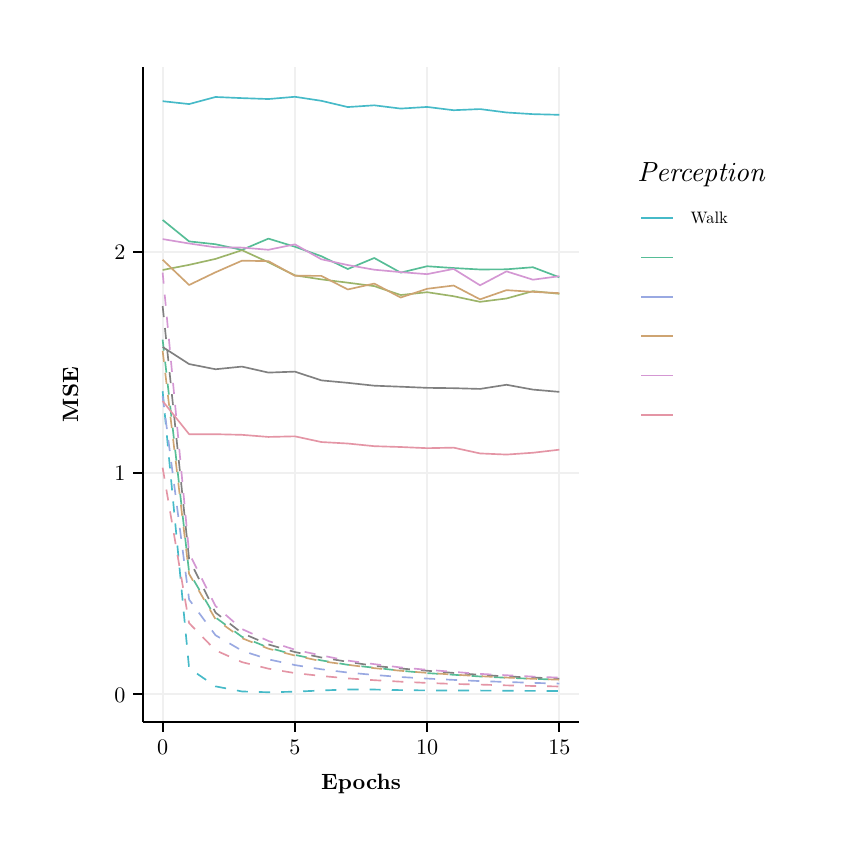
\begin{tikzpicture}[x=1pt,y=1pt]
\definecolor{fillColor}{RGB}{255,255,255}
\path[use as bounding box,fill=fillColor,fill opacity=0.00] (0,0) rectangle (289.08,289.08);
\begin{scope}
\path[clip] (  0.00,  0.00) rectangle (289.08,289.08);
\definecolor{fillColor}{RGB}{255,255,255}

\path[fill=fillColor] (  0.00,  0.00) rectangle (289.08,289.08);
\end{scope}
\begin{scope}
\path[clip] ( 41.60, 38.17) rectangle (199.30,274.85);
\definecolor{fillColor}{RGB}{255,255,255}

\path[fill=fillColor] ( 41.60, 38.17) rectangle (199.30,274.85);
\definecolor{drawColor}{gray}{0.94}

\path[draw=drawColor,line width= 0.7pt,line join=round] ( 41.60, 48.17) --
	(199.30, 48.17);

\path[draw=drawColor,line width= 0.7pt,line join=round] ( 41.60,128.16) --
	(199.30,128.16);

\path[draw=drawColor,line width= 0.7pt,line join=round] ( 41.60,208.16) --
	(199.30,208.16);

\path[draw=drawColor,line width= 0.7pt,line join=round] ( 48.77, 38.17) --
	( 48.77,274.85);

\path[draw=drawColor,line width= 0.7pt,line join=round] ( 96.56, 38.17) --
	( 96.56,274.85);

\path[draw=drawColor,line width= 0.7pt,line join=round] (144.34, 38.17) --
	(144.34,274.85);

\path[draw=drawColor,line width= 0.7pt,line join=round] (192.13, 38.17) --
	(192.13,274.85);
\definecolor{drawColor}{RGB}{70,186,200}

\path[draw=drawColor,line width= 0.6pt,dash pattern=on 4pt off 4pt ,line join=round] ( 48.77,157.70) --
	( 58.33, 57.62) --
	( 67.88, 51.06) --
	( 77.44, 49.22) --
	( 87.00, 48.93) --
	( 96.56, 49.14) --
	(106.11, 49.57) --
	(115.67, 49.94) --
	(125.23, 49.91) --
	(134.79, 49.70) --
	(144.34, 49.59) --
	(153.90, 49.54) --
	(163.46, 49.54) --
	(173.02, 49.46) --
	(182.57, 49.43) --
	(192.13, 49.40);

\path[draw=drawColor,line width= 0.6pt,line join=round] ( 48.77,262.51) --
	( 58.33,261.47) --
	( 67.88,264.03) --
	( 77.44,263.62) --
	( 87.00,263.29) --
	( 96.56,264.10) --
	(106.11,262.65) --
	(115.67,260.39) --
	(125.23,261.02) --
	(134.79,259.84) --
	(144.34,260.43) --
	(153.90,259.25) --
	(163.46,259.66) --
	(173.02,258.43) --
	(182.57,257.83) --
	(192.13,257.59);
\definecolor{drawColor}{RGB}{86,189,150}

\path[draw=drawColor,line width= 0.6pt,dash pattern=on 4pt off 4pt ,line join=round] ( 48.77,176.34) --
	( 58.33, 92.29) --
	( 67.88, 75.96) --
	( 77.44, 68.96) --
	( 87.00, 65.04) --
	( 96.56, 62.43) --
	(106.11, 60.45) --
	(115.67, 58.85) --
	(125.23, 57.80) --
	(134.79, 56.71) --
	(144.34, 55.85) --
	(153.90, 55.25) --
	(163.46, 54.64) --
	(173.02, 54.17) --
	(182.57, 53.80) --
	(192.13, 53.45);

\path[draw=drawColor,line width= 0.6pt,line join=round] ( 48.77,219.60) --
	( 58.33,211.85) --
	( 67.88,210.82) --
	( 77.44,208.78) --
	( 87.00,212.85) --
	( 96.56,209.92) --
	(106.11,206.50) --
	(115.67,201.86) --
	(125.23,205.85) --
	(134.79,200.56) --
	(144.34,202.87) --
	(153.90,202.22) --
	(163.46,201.70) --
	(173.02,201.76) --
	(182.57,202.51) --
	(192.13,198.88);
\definecolor{drawColor}{RGB}{153,169,226}

\path[draw=drawColor,line width= 0.6pt,dash pattern=on 4pt off 4pt ,line join=round] ( 48.77,155.93) --
	( 58.33, 82.44) --
	( 67.88, 69.53) --
	( 77.44, 63.95) --
	( 87.00, 60.82) --
	( 96.56, 58.76) --
	(106.11, 57.24) --
	(115.67, 56.05) --
	(125.23, 55.19) --
	(134.79, 54.44) --
	(144.34, 53.88) --
	(153.90, 53.40) --
	(163.46, 52.97) --
	(173.02, 52.65) --
	(182.57, 52.33) --
	(192.13, 52.05);
\definecolor{drawColor}{gray}{0.50}

\path[draw=drawColor,line width= 0.6pt,line join=round] ( 48.77,173.69) --
	( 58.33,167.53) --
	( 67.88,165.65) --
	( 77.44,166.61) --
	( 87.00,164.44) --
	( 96.56,164.79) --
	(106.11,161.63) --
	(115.67,160.74) --
	(125.23,159.71) --
	(134.79,159.34) --
	(144.34,158.93) --
	(153.90,158.81) --
	(163.46,158.54) --
	(173.02,160.04) --
	(182.57,158.30) --
	(192.13,157.47);

\path[draw=drawColor,line width= 0.6pt,dash pattern=on 4pt off 4pt ,line join=round] ( 48.77,188.49) --
	( 58.33, 97.08) --
	( 67.88, 77.72) --
	( 77.44, 70.32) --
	( 87.00, 66.20) --
	( 96.56, 63.47) --
	(106.11, 61.50) --
	(115.67, 59.94) --
	(125.23, 58.47) --
	(134.79, 57.52) --
	(144.34, 56.71) --
	(153.90, 55.92) --
	(163.46, 55.24) --
	(173.02, 54.64) --
	(182.57, 54.28) --
	(192.13, 53.82);
\definecolor{drawColor}{RGB}{156,180,105}

\path[draw=drawColor,line width= 0.6pt,line join=round] ( 48.77,201.52) --
	( 58.33,203.37) --
	( 67.88,205.52) --
	( 77.44,208.67) --
	( 87.00,204.30) --
	( 96.56,199.58) --
	(106.11,198.12) --
	(115.67,196.93) --
	(125.23,195.69) --
	(134.79,192.47) --
	(144.34,193.49) --
	(153.90,192.04) --
	(163.46,190.01) --
	(173.02,191.22) --
	(182.57,193.87) --
	(192.13,192.91);
\definecolor{drawColor}{RGB}{206,164,114}

\path[draw=drawColor,line width= 0.6pt,dash pattern=on 4pt off 4pt ,line join=round] ( 48.77,172.31) --
	( 58.33, 91.69) --
	( 67.88, 75.34) --
	( 77.44, 68.47) --
	( 87.00, 64.68) --
	( 96.56, 62.20) --
	(106.11, 60.16) --
	(115.67, 58.86) --
	(125.23, 57.64) --
	(134.79, 56.69) --
	(144.34, 55.94) --
	(153.90, 55.31) --
	(163.46, 54.74) --
	(173.02, 54.24) --
	(182.57, 53.79) --
	(192.13, 53.47);

\path[draw=drawColor,line width= 0.6pt,line join=round] ( 48.77,205.22) --
	( 58.33,196.09) --
	( 67.88,200.69) --
	( 77.44,204.88) --
	( 87.00,204.71) --
	( 96.56,199.43) --
	(106.11,199.39) --
	(115.67,194.48) --
	(125.23,196.61) --
	(134.79,191.56) --
	(144.34,194.72) --
	(153.90,195.90) --
	(163.46,190.91) --
	(173.02,194.23) --
	(182.57,193.61) --
	(192.13,193.15);
\definecolor{drawColor}{RGB}{212,151,211}

\path[draw=drawColor,line width= 0.6pt,dash pattern=on 4pt off 4pt ,line join=round] ( 48.77,200.55) --
	( 58.33, 99.20) --
	( 67.88, 80.09) --
	( 77.44, 71.77) --
	( 87.00, 67.47) --
	( 96.56, 64.29) --
	(106.11, 62.24) --
	(115.67, 60.37) --
	(125.23, 59.09) --
	(134.79, 57.89) --
	(144.34, 57.05) --
	(153.90, 56.30) --
	(163.46, 55.57) --
	(173.02, 55.08) --
	(182.57, 54.59) --
	(192.13, 54.21);

\path[draw=drawColor,line width= 0.6pt,line join=round] ( 48.77,212.68) --
	( 58.33,211.09) --
	( 67.88,209.72) --
	( 77.44,209.61) --
	( 87.00,208.82) --
	( 96.56,210.78) --
	(106.11,205.39) --
	(115.67,203.30) --
	(125.23,201.62) --
	(134.79,200.74) --
	(144.34,200.01) --
	(153.90,201.91) --
	(163.46,195.98) --
	(173.02,201.02) --
	(182.57,198.01) --
	(192.13,199.27);
\definecolor{drawColor}{RGB}{228,149,165}

\path[draw=drawColor,line width= 0.6pt,dash pattern=on 4pt off 4pt ,line join=round] ( 48.77,130.07) --
	( 58.33, 73.92) --
	( 67.88, 64.09) --
	( 77.44, 59.82) --
	( 87.00, 57.46) --
	( 96.56, 55.86) --
	(106.11, 54.82) --
	(115.67, 53.94) --
	(125.23, 53.29) --
	(134.79, 52.76) --
	(144.34, 52.30) --
	(153.90, 51.94) --
	(163.46, 51.70) --
	(173.02, 51.42) --
	(182.57, 51.20) --
	(192.13, 51.02);

\path[draw=drawColor,line width= 0.6pt,line join=round] ( 48.77,154.16) --
	( 58.33,142.19) --
	( 67.88,142.18) --
	( 77.44,141.95) --
	( 87.00,141.19) --
	( 96.56,141.41) --
	(106.11,139.35) --
	(115.67,138.81) --
	(125.23,137.85) --
	(134.79,137.55) --
	(144.34,137.13) --
	(153.90,137.32) --
	(163.46,135.23) --
	(173.02,134.82) --
	(182.57,135.48) --
	(192.13,136.58);

\path[] ( 41.60, 38.17) rectangle (199.30,274.85);
\end{scope}
\begin{scope}
\path[clip] (  0.00,  0.00) rectangle (289.08,289.08);
\definecolor{drawColor}{RGB}{0,0,0}

\path[draw=drawColor,line width= 0.7pt,line join=round] ( 41.60, 38.17) --
	( 41.60,274.85);
\end{scope}
\begin{scope}
\path[clip] (  0.00,  0.00) rectangle (289.08,289.08);
\definecolor{drawColor}{RGB}{0,0,0}

\node[text=drawColor,anchor=base east,inner sep=0pt, outer sep=0pt, scale=  0.80] at ( 35.30, 45.41) {0};

\node[text=drawColor,anchor=base east,inner sep=0pt, outer sep=0pt, scale=  0.80] at ( 35.30,125.41) {1};

\node[text=drawColor,anchor=base east,inner sep=0pt, outer sep=0pt, scale=  0.80] at ( 35.30,205.40) {2};
\end{scope}
\begin{scope}
\path[clip] (  0.00,  0.00) rectangle (289.08,289.08);
\definecolor{drawColor}{RGB}{0,0,0}

\path[draw=drawColor,line width= 0.7pt,line join=round] ( 38.10, 48.17) --
	( 41.60, 48.17);

\path[draw=drawColor,line width= 0.7pt,line join=round] ( 38.10,128.16) --
	( 41.60,128.16);

\path[draw=drawColor,line width= 0.7pt,line join=round] ( 38.10,208.16) --
	( 41.60,208.16);
\end{scope}
\begin{scope}
\path[clip] (  0.00,  0.00) rectangle (289.08,289.08);
\definecolor{drawColor}{RGB}{0,0,0}

\path[draw=drawColor,line width= 0.7pt,line join=round] ( 41.60, 38.17) --
	(199.30, 38.17);
\end{scope}
\begin{scope}
\path[clip] (  0.00,  0.00) rectangle (289.08,289.08);
\definecolor{drawColor}{RGB}{0,0,0}

\path[draw=drawColor,line width= 0.7pt,line join=round] ( 48.77, 34.67) --
	( 48.77, 38.17);

\path[draw=drawColor,line width= 0.7pt,line join=round] ( 96.56, 34.67) --
	( 96.56, 38.17);

\path[draw=drawColor,line width= 0.7pt,line join=round] (144.34, 34.67) --
	(144.34, 38.17);

\path[draw=drawColor,line width= 0.7pt,line join=round] (192.13, 34.67) --
	(192.13, 38.17);
\end{scope}
\begin{scope}
\path[clip] (  0.00,  0.00) rectangle (289.08,289.08);
\definecolor{drawColor}{RGB}{0,0,0}

\node[text=drawColor,anchor=base,inner sep=0pt, outer sep=0pt, scale=  0.80] at ( 48.77, 26.36) {0};

\node[text=drawColor,anchor=base,inner sep=0pt, outer sep=0pt, scale=  0.80] at ( 96.56, 26.36) {5};

\node[text=drawColor,anchor=base,inner sep=0pt, outer sep=0pt, scale=  0.80] at (144.34, 26.36) {10};

\node[text=drawColor,anchor=base,inner sep=0pt, outer sep=0pt, scale=  0.80] at (192.13, 26.36) {15};
\end{scope}
\begin{scope}
\path[clip] (  0.00,  0.00) rectangle (289.08,289.08);
\definecolor{drawColor}{RGB}{0,0,0}

\node[text=drawColor,anchor=base,inner sep=0pt, outer sep=0pt, scale=  0.80] at (120.45, 13.92) {\bfseries Epochs};
\end{scope}
\begin{scope}
\path[clip] (  0.00,  0.00) rectangle (289.08,289.08);
\definecolor{drawColor}{RGB}{0,0,0}

\node[text=drawColor,rotate= 90.00,anchor=base,inner sep=0pt, outer sep=0pt, scale=  0.80] at ( 18.19,156.51) {\bfseries MSE};
\end{scope}
\begin{scope}
\path[clip] (  0.00,  0.00) rectangle (289.08,289.08);
\definecolor{fillColor}{RGB}{255,255,255}

\path[fill=fillColor] (213.30,135.06) rectangle (274.85,248.25);
\end{scope}
\begin{scope}
\path[clip] (  0.00,  0.00) rectangle (289.08,289.08);
\definecolor{drawColor}{RGB}{0,0,0}

\node[text=drawColor,anchor=base west,inner sep=0pt, outer sep=0pt, scale=  1.00] at (220.30,233.39) {\itshape Perception};
\end{scope}
\begin{scope}
\path[clip] (  0.00,  0.00) rectangle (289.08,289.08);
\definecolor{fillColor}{RGB}{255,255,255}

\path[fill=fillColor] (220.30,213.19) rectangle (234.53,227.42);
\end{scope}
\begin{scope}
\path[clip] (  0.00,  0.00) rectangle (289.08,289.08);
\definecolor{drawColor}{RGB}{70,186,200}

\path[draw=drawColor,line width= 0.6pt,line join=round] (221.72,220.30) -- (233.10,220.30);
\end{scope}
\begin{scope}
\path[clip] (  0.00,  0.00) rectangle (289.08,289.08);
\definecolor{fillColor}{RGB}{255,255,255}

\path[fill=fillColor] (220.30,198.96) rectangle (234.53,213.19);
\end{scope}
\begin{scope}
\path[clip] (  0.00,  0.00) rectangle (289.08,289.08);
\definecolor{drawColor}{RGB}{86,189,150}

\path[draw=drawColor,line width= 0.6pt,line join=round] (221.72,206.08) -- (233.10,206.08);
\end{scope}
\begin{scope}
\path[clip] (  0.00,  0.00) rectangle (289.08,289.08);
\definecolor{fillColor}{RGB}{255,255,255}

\path[fill=fillColor] (220.30,184.74) rectangle (234.53,198.96);
\end{scope}
\begin{scope}
\path[clip] (  0.00,  0.00) rectangle (289.08,289.08);
\definecolor{drawColor}{RGB}{153,169,226}

\path[draw=drawColor,line width= 0.6pt,line join=round] (221.72,191.85) -- (233.10,191.85);
\end{scope}
\begin{scope}
\path[clip] (  0.00,  0.00) rectangle (289.08,289.08);
\definecolor{fillColor}{RGB}{255,255,255}

\path[fill=fillColor] (220.30,170.51) rectangle (234.53,184.74);
\end{scope}
\begin{scope}
\path[clip] (  0.00,  0.00) rectangle (289.08,289.08);
\definecolor{drawColor}{RGB}{206,164,114}

\path[draw=drawColor,line width= 0.6pt,line join=round] (221.72,177.62) -- (233.10,177.62);
\end{scope}
\begin{scope}
\path[clip] (  0.00,  0.00) rectangle (289.08,289.08);
\definecolor{fillColor}{RGB}{255,255,255}

\path[fill=fillColor] (220.30,156.28) rectangle (234.53,170.51);
\end{scope}
\begin{scope}
\path[clip] (  0.00,  0.00) rectangle (289.08,289.08);
\definecolor{drawColor}{RGB}{212,151,211}

\path[draw=drawColor,line width= 0.6pt,line join=round] (221.72,163.40) -- (233.10,163.40);
\end{scope}
\begin{scope}
\path[clip] (  0.00,  0.00) rectangle (289.08,289.08);
\definecolor{fillColor}{RGB}{255,255,255}

\path[fill=fillColor] (220.30,142.06) rectangle (234.53,156.28);
\end{scope}
\begin{scope}
\path[clip] (  0.00,  0.00) rectangle (289.08,289.08);
\definecolor{drawColor}{RGB}{228,149,165}

\path[draw=drawColor,line width= 0.6pt,line join=round] (221.72,149.17) -- (233.10,149.17);
\end{scope}
\begin{scope}
\path[clip] (  0.00,  0.00) rectangle (289.08,289.08);
\definecolor{drawColor}{RGB}{0,0,0}

\node[text=drawColor,anchor=base west,inner sep=0pt, outer sep=0pt, scale=  0.60] at (239.53,218.24) {Walk};
\end{scope}
\end{tikzpicture}
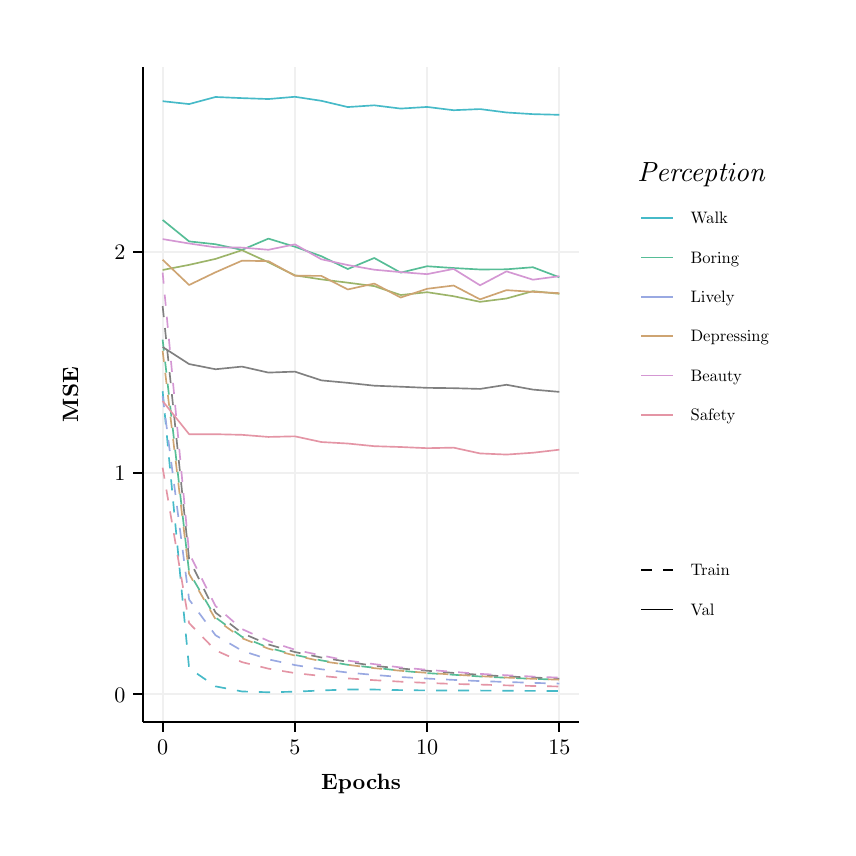
\begin{tikzpicture}[x=1pt,y=1pt]
\definecolor{fillColor}{RGB}{255,255,255}
\path[use as bounding box,fill=fillColor,fill opacity=0.00] (0,0) rectangle (289.08,289.08);
\begin{scope}
\path[clip] (  0.00,  0.00) rectangle (289.08,289.08);
\definecolor{fillColor}{RGB}{255,255,255}

\path[fill=fillColor] (  0.00,  0.00) rectangle (289.08,289.08);
\end{scope}
\begin{scope}
\path[clip] ( 41.60, 38.17) rectangle (199.30,274.85);
\definecolor{fillColor}{RGB}{255,255,255}

\path[fill=fillColor] ( 41.60, 38.17) rectangle (199.30,274.85);
\definecolor{drawColor}{gray}{0.94}

\path[draw=drawColor,line width= 0.7pt,line join=round] ( 41.60, 48.17) --
	(199.30, 48.17);

\path[draw=drawColor,line width= 0.7pt,line join=round] ( 41.60,128.16) --
	(199.30,128.16);

\path[draw=drawColor,line width= 0.7pt,line join=round] ( 41.60,208.16) --
	(199.30,208.16);

\path[draw=drawColor,line width= 0.7pt,line join=round] ( 48.77, 38.17) --
	( 48.77,274.85);

\path[draw=drawColor,line width= 0.7pt,line join=round] ( 96.56, 38.17) --
	( 96.56,274.85);

\path[draw=drawColor,line width= 0.7pt,line join=round] (144.34, 38.17) --
	(144.34,274.85);

\path[draw=drawColor,line width= 0.7pt,line join=round] (192.13, 38.17) --
	(192.13,274.85);
\definecolor{drawColor}{RGB}{70,186,200}

\path[draw=drawColor,line width= 0.6pt,dash pattern=on 4pt off 4pt ,line join=round] ( 48.77,157.70) --
	( 58.33, 57.62) --
	( 67.88, 51.06) --
	( 77.44, 49.22) --
	( 87.00, 48.93) --
	( 96.56, 49.14) --
	(106.11, 49.57) --
	(115.67, 49.94) --
	(125.23, 49.91) --
	(134.79, 49.70) --
	(144.34, 49.59) --
	(153.90, 49.54) --
	(163.46, 49.54) --
	(173.02, 49.46) --
	(182.57, 49.43) --
	(192.13, 49.40);

\path[draw=drawColor,line width= 0.6pt,line join=round] ( 48.77,262.51) --
	( 58.33,261.47) --
	( 67.88,264.03) --
	( 77.44,263.62) --
	( 87.00,263.29) --
	( 96.56,264.10) --
	(106.11,262.65) --
	(115.67,260.39) --
	(125.23,261.02) --
	(134.79,259.84) --
	(144.34,260.43) --
	(153.90,259.25) --
	(163.46,259.66) --
	(173.02,258.43) --
	(182.57,257.83) --
	(192.13,257.59);
\definecolor{drawColor}{RGB}{86,189,150}

\path[draw=drawColor,line width= 0.6pt,dash pattern=on 4pt off 4pt ,line join=round] ( 48.77,176.34) --
	( 58.33, 92.29) --
	( 67.88, 75.96) --
	( 77.44, 68.96) --
	( 87.00, 65.04) --
	( 96.56, 62.43) --
	(106.11, 60.45) --
	(115.67, 58.85) --
	(125.23, 57.80) --
	(134.79, 56.71) --
	(144.34, 55.85) --
	(153.90, 55.25) --
	(163.46, 54.64) --
	(173.02, 54.17) --
	(182.57, 53.80) --
	(192.13, 53.45);

\path[draw=drawColor,line width= 0.6pt,line join=round] ( 48.77,219.60) --
	( 58.33,211.85) --
	( 67.88,210.82) --
	( 77.44,208.78) --
	( 87.00,212.85) --
	( 96.56,209.92) --
	(106.11,206.50) --
	(115.67,201.86) --
	(125.23,205.85) --
	(134.79,200.56) --
	(144.34,202.87) --
	(153.90,202.22) --
	(163.46,201.70) --
	(173.02,201.76) --
	(182.57,202.51) --
	(192.13,198.88);
\definecolor{drawColor}{RGB}{153,169,226}

\path[draw=drawColor,line width= 0.6pt,dash pattern=on 4pt off 4pt ,line join=round] ( 48.77,155.93) --
	( 58.33, 82.44) --
	( 67.88, 69.53) --
	( 77.44, 63.95) --
	( 87.00, 60.82) --
	( 96.56, 58.76) --
	(106.11, 57.24) --
	(115.67, 56.05) --
	(125.23, 55.19) --
	(134.79, 54.44) --
	(144.34, 53.88) --
	(153.90, 53.40) --
	(163.46, 52.97) --
	(173.02, 52.65) --
	(182.57, 52.33) --
	(192.13, 52.05);
\definecolor{drawColor}{gray}{0.50}

\path[draw=drawColor,line width= 0.6pt,line join=round] ( 48.77,173.69) --
	( 58.33,167.53) --
	( 67.88,165.65) --
	( 77.44,166.61) --
	( 87.00,164.44) --
	( 96.56,164.79) --
	(106.11,161.63) --
	(115.67,160.74) --
	(125.23,159.71) --
	(134.79,159.34) --
	(144.34,158.93) --
	(153.90,158.81) --
	(163.46,158.54) --
	(173.02,160.04) --
	(182.57,158.30) --
	(192.13,157.47);

\path[draw=drawColor,line width= 0.6pt,dash pattern=on 4pt off 4pt ,line join=round] ( 48.77,188.49) --
	( 58.33, 97.08) --
	( 67.88, 77.72) --
	( 77.44, 70.32) --
	( 87.00, 66.20) --
	( 96.56, 63.47) --
	(106.11, 61.50) --
	(115.67, 59.94) --
	(125.23, 58.47) --
	(134.79, 57.52) --
	(144.34, 56.71) --
	(153.90, 55.92) --
	(163.46, 55.24) --
	(173.02, 54.64) --
	(182.57, 54.28) --
	(192.13, 53.82);
\definecolor{drawColor}{RGB}{156,180,105}

\path[draw=drawColor,line width= 0.6pt,line join=round] ( 48.77,201.52) --
	( 58.33,203.37) --
	( 67.88,205.52) --
	( 77.44,208.67) --
	( 87.00,204.30) --
	( 96.56,199.58) --
	(106.11,198.12) --
	(115.67,196.93) --
	(125.23,195.69) --
	(134.79,192.47) --
	(144.34,193.49) --
	(153.90,192.04) --
	(163.46,190.01) --
	(173.02,191.22) --
	(182.57,193.87) --
	(192.13,192.91);
\definecolor{drawColor}{RGB}{206,164,114}

\path[draw=drawColor,line width= 0.6pt,dash pattern=on 4pt off 4pt ,line join=round] ( 48.77,172.31) --
	( 58.33, 91.69) --
	( 67.88, 75.34) --
	( 77.44, 68.47) --
	( 87.00, 64.68) --
	( 96.56, 62.20) --
	(106.11, 60.16) --
	(115.67, 58.86) --
	(125.23, 57.64) --
	(134.79, 56.69) --
	(144.34, 55.94) --
	(153.90, 55.31) --
	(163.46, 54.74) --
	(173.02, 54.24) --
	(182.57, 53.79) --
	(192.13, 53.47);

\path[draw=drawColor,line width= 0.6pt,line join=round] ( 48.77,205.22) --
	( 58.33,196.09) --
	( 67.88,200.69) --
	( 77.44,204.88) --
	( 87.00,204.71) --
	( 96.56,199.43) --
	(106.11,199.39) --
	(115.67,194.48) --
	(125.23,196.61) --
	(134.79,191.56) --
	(144.34,194.72) --
	(153.90,195.90) --
	(163.46,190.91) --
	(173.02,194.23) --
	(182.57,193.61) --
	(192.13,193.15);
\definecolor{drawColor}{RGB}{212,151,211}

\path[draw=drawColor,line width= 0.6pt,dash pattern=on 4pt off 4pt ,line join=round] ( 48.77,200.55) --
	( 58.33, 99.20) --
	( 67.88, 80.09) --
	( 77.44, 71.77) --
	( 87.00, 67.47) --
	( 96.56, 64.29) --
	(106.11, 62.24) --
	(115.67, 60.37) --
	(125.23, 59.09) --
	(134.79, 57.89) --
	(144.34, 57.05) --
	(153.90, 56.30) --
	(163.46, 55.57) --
	(173.02, 55.08) --
	(182.57, 54.59) --
	(192.13, 54.21);

\path[draw=drawColor,line width= 0.6pt,line join=round] ( 48.77,212.68) --
	( 58.33,211.09) --
	( 67.88,209.72) --
	( 77.44,209.61) --
	( 87.00,208.82) --
	( 96.56,210.78) --
	(106.11,205.39) --
	(115.67,203.30) --
	(125.23,201.62) --
	(134.79,200.74) --
	(144.34,200.01) --
	(153.90,201.91) --
	(163.46,195.98) --
	(173.02,201.02) --
	(182.57,198.01) --
	(192.13,199.27);
\definecolor{drawColor}{RGB}{228,149,165}

\path[draw=drawColor,line width= 0.6pt,dash pattern=on 4pt off 4pt ,line join=round] ( 48.77,130.07) --
	( 58.33, 73.92) --
	( 67.88, 64.09) --
	( 77.44, 59.82) --
	( 87.00, 57.46) --
	( 96.56, 55.86) --
	(106.11, 54.82) --
	(115.67, 53.94) --
	(125.23, 53.29) --
	(134.79, 52.76) --
	(144.34, 52.30) --
	(153.90, 51.94) --
	(163.46, 51.70) --
	(173.02, 51.42) --
	(182.57, 51.20) --
	(192.13, 51.02);

\path[draw=drawColor,line width= 0.6pt,line join=round] ( 48.77,154.16) --
	( 58.33,142.19) --
	( 67.88,142.18) --
	( 77.44,141.95) --
	( 87.00,141.19) --
	( 96.56,141.41) --
	(106.11,139.35) --
	(115.67,138.81) --
	(125.23,137.85) --
	(134.79,137.55) --
	(144.34,137.13) --
	(153.90,137.32) --
	(163.46,135.23) --
	(173.02,134.82) --
	(182.57,135.48) --
	(192.13,136.58);

\path[] ( 41.60, 38.17) rectangle (199.30,274.85);
\end{scope}
\begin{scope}
\path[clip] (  0.00,  0.00) rectangle (289.08,289.08);
\definecolor{drawColor}{RGB}{0,0,0}

\path[draw=drawColor,line width= 0.7pt,line join=round] ( 41.60, 38.17) --
	( 41.60,274.85);
\end{scope}
\begin{scope}
\path[clip] (  0.00,  0.00) rectangle (289.08,289.08);
\definecolor{drawColor}{RGB}{0,0,0}

\node[text=drawColor,anchor=base east,inner sep=0pt, outer sep=0pt, scale=  0.80] at ( 35.30, 45.41) {0};

\node[text=drawColor,anchor=base east,inner sep=0pt, outer sep=0pt, scale=  0.80] at ( 35.30,125.41) {1};

\node[text=drawColor,anchor=base east,inner sep=0pt, outer sep=0pt, scale=  0.80] at ( 35.30,205.40) {2};
\end{scope}
\begin{scope}
\path[clip] (  0.00,  0.00) rectangle (289.08,289.08);
\definecolor{drawColor}{RGB}{0,0,0}

\path[draw=drawColor,line width= 0.7pt,line join=round] ( 38.10, 48.17) --
	( 41.60, 48.17);

\path[draw=drawColor,line width= 0.7pt,line join=round] ( 38.10,128.16) --
	( 41.60,128.16);

\path[draw=drawColor,line width= 0.7pt,line join=round] ( 38.10,208.16) --
	( 41.60,208.16);
\end{scope}
\begin{scope}
\path[clip] (  0.00,  0.00) rectangle (289.08,289.08);
\definecolor{drawColor}{RGB}{0,0,0}

\path[draw=drawColor,line width= 0.7pt,line join=round] ( 41.60, 38.17) --
	(199.30, 38.17);
\end{scope}
\begin{scope}
\path[clip] (  0.00,  0.00) rectangle (289.08,289.08);
\definecolor{drawColor}{RGB}{0,0,0}

\path[draw=drawColor,line width= 0.7pt,line join=round] ( 48.77, 34.67) --
	( 48.77, 38.17);

\path[draw=drawColor,line width= 0.7pt,line join=round] ( 96.56, 34.67) --
	( 96.56, 38.17);

\path[draw=drawColor,line width= 0.7pt,line join=round] (144.34, 34.67) --
	(144.34, 38.17);

\path[draw=drawColor,line width= 0.7pt,line join=round] (192.13, 34.67) --
	(192.13, 38.17);
\end{scope}
\begin{scope}
\path[clip] (  0.00,  0.00) rectangle (289.08,289.08);
\definecolor{drawColor}{RGB}{0,0,0}

\node[text=drawColor,anchor=base,inner sep=0pt, outer sep=0pt, scale=  0.80] at ( 48.77, 26.36) {0};

\node[text=drawColor,anchor=base,inner sep=0pt, outer sep=0pt, scale=  0.80] at ( 96.56, 26.36) {5};

\node[text=drawColor,anchor=base,inner sep=0pt, outer sep=0pt, scale=  0.80] at (144.34, 26.36) {10};

\node[text=drawColor,anchor=base,inner sep=0pt, outer sep=0pt, scale=  0.80] at (192.13, 26.36) {15};
\end{scope}
\begin{scope}
\path[clip] (  0.00,  0.00) rectangle (289.08,289.08);
\definecolor{drawColor}{RGB}{0,0,0}

\node[text=drawColor,anchor=base,inner sep=0pt, outer sep=0pt, scale=  0.80] at (120.45, 13.92) {\bfseries Epochs};
\end{scope}
\begin{scope}
\path[clip] (  0.00,  0.00) rectangle (289.08,289.08);
\definecolor{drawColor}{RGB}{0,0,0}

\node[text=drawColor,rotate= 90.00,anchor=base,inner sep=0pt, outer sep=0pt, scale=  0.80] at ( 18.19,156.51) {\bfseries MSE};
\end{scope}
\begin{scope}
\path[clip] (  0.00,  0.00) rectangle (289.08,289.08);
\definecolor{fillColor}{RGB}{255,255,255}

\path[fill=fillColor] (213.30,135.06) rectangle (274.85,248.25);
\end{scope}
\begin{scope}
\path[clip] (  0.00,  0.00) rectangle (289.08,289.08);
\definecolor{drawColor}{RGB}{0,0,0}

\node[text=drawColor,anchor=base west,inner sep=0pt, outer sep=0pt, scale=  1.00] at (220.30,233.39) {\itshape Perception};
\end{scope}
\begin{scope}
\path[clip] (  0.00,  0.00) rectangle (289.08,289.08);
\definecolor{fillColor}{RGB}{255,255,255}

\path[fill=fillColor] (220.30,213.19) rectangle (234.53,227.42);
\end{scope}
\begin{scope}
\path[clip] (  0.00,  0.00) rectangle (289.08,289.08);
\definecolor{drawColor}{RGB}{70,186,200}

\path[draw=drawColor,line width= 0.6pt,line join=round] (221.72,220.30) -- (233.10,220.30);
\end{scope}
\begin{scope}
\path[clip] (  0.00,  0.00) rectangle (289.08,289.08);
\definecolor{fillColor}{RGB}{255,255,255}

\path[fill=fillColor] (220.30,198.96) rectangle (234.53,213.19);
\end{scope}
\begin{scope}
\path[clip] (  0.00,  0.00) rectangle (289.08,289.08);
\definecolor{drawColor}{RGB}{86,189,150}

\path[draw=drawColor,line width= 0.6pt,line join=round] (221.72,206.08) -- (233.10,206.08);
\end{scope}
\begin{scope}
\path[clip] (  0.00,  0.00) rectangle (289.08,289.08);
\definecolor{fillColor}{RGB}{255,255,255}

\path[fill=fillColor] (220.30,184.74) rectangle (234.53,198.96);
\end{scope}
\begin{scope}
\path[clip] (  0.00,  0.00) rectangle (289.08,289.08);
\definecolor{drawColor}{RGB}{153,169,226}

\path[draw=drawColor,line width= 0.6pt,line join=round] (221.72,191.85) -- (233.10,191.85);
\end{scope}
\begin{scope}
\path[clip] (  0.00,  0.00) rectangle (289.08,289.08);
\definecolor{fillColor}{RGB}{255,255,255}

\path[fill=fillColor] (220.30,170.51) rectangle (234.53,184.74);
\end{scope}
\begin{scope}
\path[clip] (  0.00,  0.00) rectangle (289.08,289.08);
\definecolor{drawColor}{RGB}{206,164,114}

\path[draw=drawColor,line width= 0.6pt,line join=round] (221.72,177.62) -- (233.10,177.62);
\end{scope}
\begin{scope}
\path[clip] (  0.00,  0.00) rectangle (289.08,289.08);
\definecolor{fillColor}{RGB}{255,255,255}

\path[fill=fillColor] (220.30,156.28) rectangle (234.53,170.51);
\end{scope}
\begin{scope}
\path[clip] (  0.00,  0.00) rectangle (289.08,289.08);
\definecolor{drawColor}{RGB}{212,151,211}

\path[draw=drawColor,line width= 0.6pt,line join=round] (221.72,163.40) -- (233.10,163.40);
\end{scope}
\begin{scope}
\path[clip] (  0.00,  0.00) rectangle (289.08,289.08);
\definecolor{fillColor}{RGB}{255,255,255}

\path[fill=fillColor] (220.30,142.06) rectangle (234.53,156.28);
\end{scope}
\begin{scope}
\path[clip] (  0.00,  0.00) rectangle (289.08,289.08);
\definecolor{drawColor}{RGB}{228,149,165}

\path[draw=drawColor,line width= 0.6pt,line join=round] (221.72,149.17) -- (233.10,149.17);
\end{scope}
\begin{scope}
\path[clip] (  0.00,  0.00) rectangle (289.08,289.08);
\definecolor{drawColor}{RGB}{0,0,0}

\node[text=drawColor,anchor=base west,inner sep=0pt, outer sep=0pt, scale=  0.60] at (239.53,218.24) {Walk};
\end{scope}
\begin{scope}
\path[clip] (  0.00,  0.00) rectangle (289.08,289.08);
\definecolor{drawColor}{RGB}{0,0,0}

\node[text=drawColor,anchor=base west,inner sep=0pt, outer sep=0pt, scale=  0.60] at (239.53,204.01) {Boring};
\end{scope}
\begin{scope}
\path[clip] (  0.00,  0.00) rectangle (289.08,289.08);
\definecolor{drawColor}{RGB}{0,0,0}

\node[text=drawColor,anchor=base west,inner sep=0pt, outer sep=0pt, scale=  0.60] at (239.53,189.78) {Lively};
\end{scope}
\begin{scope}
\path[clip] (  0.00,  0.00) rectangle (289.08,289.08);
\definecolor{drawColor}{RGB}{0,0,0}

\node[text=drawColor,anchor=base west,inner sep=0pt, outer sep=0pt, scale=  0.60] at (239.53,175.56) {Depressing};
\end{scope}
\begin{scope}
\path[clip] (  0.00,  0.00) rectangle (289.08,289.08);
\definecolor{drawColor}{RGB}{0,0,0}

\node[text=drawColor,anchor=base west,inner sep=0pt, outer sep=0pt, scale=  0.60] at (239.53,161.33) {Beauty};
\end{scope}
\begin{scope}
\path[clip] (  0.00,  0.00) rectangle (289.08,289.08);
\definecolor{drawColor}{RGB}{0,0,0}

\node[text=drawColor,anchor=base west,inner sep=0pt, outer sep=0pt, scale=  0.60] at (239.53,147.10) {Safety};
\end{scope}
\begin{scope}
\path[clip] (  0.00,  0.00) rectangle (289.08,289.08);
\definecolor{fillColor}{RGB}{255,255,255}

\path[fill=fillColor] (213.30, 64.77) rectangle (260.71,121.06);
\end{scope}
\begin{scope}
\path[clip] (  0.00,  0.00) rectangle (289.08,289.08);
\definecolor{drawColor}{RGB}{0,0,0}

\node[text=drawColor,anchor=base west,inner sep=0pt, outer sep=0pt, scale=  1.00] at (220.30,106.20) {\itshape  };
\end{scope}
\begin{scope}
\path[clip] (  0.00,  0.00) rectangle (289.08,289.08);
\definecolor{fillColor}{RGB}{255,255,255}

\path[fill=fillColor] (220.30, 86.00) rectangle (234.53,100.23);
\end{scope}
\begin{scope}
\path[clip] (  0.00,  0.00) rectangle (289.08,289.08);
\definecolor{drawColor}{RGB}{0,0,0}

\path[draw=drawColor,line width= 0.6pt,dash pattern=on 4pt off 4pt ,line join=round] (221.72, 93.11) -- (233.10, 93.11);
\end{scope}
\begin{scope}
\path[clip] (  0.00,  0.00) rectangle (289.08,289.08);
\definecolor{fillColor}{RGB}{255,255,255}

\path[fill=fillColor] (220.30, 71.77) rectangle (234.53, 86.00);
\end{scope}
\begin{scope}
\path[clip] (  0.00,  0.00) rectangle (289.08,289.08);
\definecolor{drawColor}{RGB}{0,0,0}

\path[draw=drawColor,line width= 0.6pt,line join=round] (221.72, 78.89) -- (233.10, 78.89);
\end{scope}
\begin{scope}
\path[clip] (  0.00,  0.00) rectangle (289.08,289.08);
\definecolor{drawColor}{RGB}{0,0,0}

\node[text=drawColor,anchor=base west,inner sep=0pt, outer sep=0pt, scale=  0.60] at (239.53, 91.05) {Train};
\end{scope}
\begin{scope}
\path[clip] (  0.00,  0.00) rectangle (289.08,289.08);
\definecolor{drawColor}{RGB}{0,0,0}

\node[text=drawColor,anchor=base west,inner sep=0pt, outer sep=0pt, scale=  0.60] at (239.53, 76.82) {Val};
\end{scope}
\end{tikzpicture}
